\documentclass[onecolumn, draftclsnofoot,10pt, compsoc]{IEEEtran}
\usepackage{url}
\usepackage[colorlinks = true,
            linkcolor = blue,
            urlcolor  = blue,
            citecolor = blue,
            anchorcolor = blue]{hyperref}
\usepackage{setspace}
\usepackage{listings}
\usepackage{graphicx}
\usepackage{pgfgantt}
\usepackage{enumerate}
\usepackage{amssymb}
\usepackage{geometry}
\usepackage[export]{adjustbox}
\geometry{textheight=9.5in, textwidth=7in}
\usepackage{subfiles}
\bibliographystyle{IEEEtran}

% 1. Fill in these details
\def \CapstoneTeamName{		COALFO}
\def \CapstoneTeamNumber{		28}
\def \GroupMemberOne{			Kenny Thompson}
\def \GroupMemberTwo{			Bryce Egley}
\def \CapstoneProjectName{		Coal and Open-pit surface mining impacts on American Lands Follow-On (COAL-FO) - Turning spectro-imagery into usable data}
\def \CapstoneSponsorCompany{	NASA JPL}
\def \CapstoneSponsorPerson{		Lewis John Mcgibbney}

% 2. Uncomment the appropriate line below so that the document type works
\def \DocType{	%Problem Statement
				%Requirements Document
				%Technology Review
				%Design Document
				Progress Report
				}

\newcommand{\NameSigPair}[1]{\par
\makebox[2.75in][r]{#1} \hfil 	\makebox[3.25in]{\makebox[2.25in]{\hrulefill} \hfill		\makebox[.75in]{\hrulefill}}
\par\vspace{-12pt} \textit{\tiny\noindent
\makebox[2.75in]{} \hfil		\makebox[3.25in]{\makebox[2.25in][r]{Signature} \hfill	\makebox[.75in][r]{Date}}}}
% 3. If the document is not to be signed, uncomment the RENEWcommand below
\renewcommand{\NameSigPair}[1]{#1}

%%%%%%%%%%%%%%%%%%%%%%%%%%%%%%%%%%%%%%%
\begin{document}
\begin{titlepage}
    \pagenumbering{gobble}
    \begin{singlespace}
    	%\includegraphics[height=4cm]{coe_v_spot1}
        \hfill
        % 4. If you have a logo, use this includegraphics command to put it on the coversheet.
        %\includegraphics[height=4cm]{CompanyLogo}
        \par\vspace{.2in}
        \centering
        \scshape{
            \huge CS Capstone \DocType \par
            {\large\today}\par
            \vspace{.5in}
            \textbf{\Huge\CapstoneProjectName}\par
            \vfill
            {\large Prepared for}\par
            \Huge \CapstoneSponsorCompany\par
            \vspace{5pt}
            {\Large\NameSigPair{\CapstoneSponsorPerson}\par}
            {\large Prepared by }\par
            Group\CapstoneTeamNumber\par
            % 5. comment out the line below this one if you do not wish to name your team
            \CapstoneTeamName\par
            \vspace{5pt}
            {\Large
                \NameSigPair{\GroupMemberOne}\par
                \NameSigPair{\GroupMemberTwo}\par
            }
            \vspace{20pt}
        }
        \begin{abstract}
        % 6. Fill in your abstract
        	Coal and Open-pit surface mining impacts on American Lands Follow-On (COAL-FO) is the successor 				project to the 2016-2017 COAL project. COAL initially aimed to deliver a suite of algorithms to identify, classify, characterize, and quantify (by reporting a number of key metrics) the direct and indirect impacts of mining operations and related destructive surface mining activities across the continental U.S (and further afield). COAL successfully delivered a Python library for processing hyperspectral imagery from remote sensing devices such as the Airborne Visible/InfraRed Imaging Spectrometer (AVIRIS) and a Science Data System for running COAL pipelines. COAL-FO will utilize recent funding obtained from a recently awarded NSF-funded XSEDE high performance computing (HPC) grant to further improve, validate and document COAL algorithms, execution runtime performance and geospatial output results.[1]
        \end{abstract}
    \end{singlespace}
\end{titlepage}
\newpage
\pagenumbering{arabic}
\tableofcontents
% 7. uncomment this (if applicable). Consider adding a page break.
%\listoffigures
%\listoftables
\clearpage

\section{PART 1: Introduction to Project}
\subsection{Who requested it?}
This project was requested by \href{https://github.com/lewismc}{Lewis John McGibbney} a Data Scientist working for the NASA Jet Propulsion Laboratory. 
\subsection{Why was it requested?}
Coal and Open-pit surface mining impacts on American Lands Follow-On (COAL-FO) is the successor 				project to the 2016-2017 COAL project. COAL initially aimed to deliver a suite of algorithms to identify, classify, characterize, and quantify (by reporting a number of key metrics) the direct and indirect impacts of mining operations and related destructive surface mining activities across the continental U.S (and further afield). COAL successfully delivered a Python library for processing hyperspectral imagery from remote sensing devices such as the Airborne Visible/InfraRed Imaging Spectrometer (AVIRIS) and a Science Data System for running COAL pipelines. COAL-FO will utilize recent funding obtained from a recently awarded NSF-funded XSEDE high performance computing (HPC) grant to further improve, validate and document COAL algorithms, execution runtime performance and geospatial output results.[1]
\subsection{What is its importance?}
Overall this project is very important since we need to track and monitor the
environmental changes and effects coal has on surrounding lands since Coal is
one of America's main sources of energy. We want to make sure we are extracting
coal and using it safely for the sake of the environment. Satellite imaging
using remote sensing devices allows us to gather much more data than a human
eye is able to. Satellite imaging can provide a picture of an entire area of
land and see things invisible to the human eye such as methane emissions.
\subsection{Who was/were your client(s)?}
The client for this project was \href{https://github.com/lewismc}{Lewis John McGibbney} a Data Scientist working for the NASA Jet Propulsion Laboratory. 
\subsection{Who are the members of your team?}
The team members for this project were Bryce Egley and Kenneth Thompson.
\subsection{What were their roles?}
Bryce Egley focused on pycoal and the website for the duration of the project. With the specific focus of building a CLI, allowing Pycoal to support USGS Spectral Library Version 7 and the EcoStress Spectral Library by creating conversion functions to convert the Spectral Libraries into a suitable file format for pycoal to use. As well as coming up with installation instructions on the website for installing GDAL and QGIS for any type of Operating System. And other smaller tasks such as finding new data and fixing existing bugs in pycoal.
\newline
Kenneth Thompson focused on COAL-SDS for the beginning of the project and then moved over to pycoal to work on the classifier callback. 
\subsection{What was the role of the client(s)? (I.e., did they supervise only, or did they participate in doing development)}
The main role of Lewis the client was supervising. Once code was submitted by Bryce and Kenneth via pull requests, Lewis would offer feedback, or make minor changes to the code before accepting it or asking for us to keep working on it.
\subfile{problem_statement}

\subsection{Project Proposal}
Coal and Open-pit surface mining impacts on American Lands Follow-On (COAL-FO) is the successor project to the 2016-2017 COAL project. COAL initially aimed to deliver a suite of algorithms to identify, classify, characterize, and quantify (by reporting a number of key metrics) the direct and indirect impacts of mining operations and related destructive surface mining activities across the continental U.S (and further afield). COAL successfully delivered a Python library for processing hyperspectral imagery from remote sensing devices such as the Airborne Visible/InfraRed Imaging Spectrometer (AVIRIS) and a Science Data System for running COAL pipelines. COAL-FO will utilize recent funding obtained from a recently awarded NSF-funded XSEDE high performance computing (HPC) grant to further improve, validate and document COAL algorithms, execution runtime performance and geospatial output results.

\section{PART 2: Requirements Document and Design Document}
\subsection{Original Requirements Document}

\subfile{RequirementsOld}

\subsection{Final Requirements Document - Client approved}

\subfile{Requirements}

\subsection{Final Gantt Chart}
\begin{ganttchart}{1}{33}
  \gantttitle{Coal-FO Capstone Gantt Chart (Every Quarter has 11 weeks, so 33 for 33 weeks)}{33} \\
  \gantttitlelist{1,...,33}{1} \\
  \ganttgroup[progress=100]{Class Intro}{1}{2}\\
  \ganttgroup[progress=100]{Problem Statement}{3}{4} \\
  \ganttgroup[progress=100]{Requirements Doc}{4}{6} \\
  \ganttgroup[progress=100]{Learning Pycoal}{7}{13} \\
  \ganttgroup[progress=100]{Tech Review}{8}{9} \\
  \ganttgroup[progress=100]{Design Doc}{9}{10} \\
  \ganttgroup[progress=100]{Update Docker}{13}{15} \\
  \ganttgroup[progress=100]{QGIS and GDAL}{15}{17} \\
  \ganttgroup[progress=100]{Alpha}{14}{15} \\
  \ganttgroup[progress=100]{AWS}{10}{15} \\
  \ganttgroup[progress=100]{Update SDS}{11}{12} \\
  \ganttgroup[progress=60]{Classifier}{11}{26} \\
  \ganttgroup[progress=100]{Create CLI}{17}{18} \\
  \ganttgroup[progress=100]{Find Data}{18}{19} \\
  \ganttgroup[progress=100]{GDAL bug}{19}{20} \\
  \ganttgroup[progress=100]{USGS Sv7}{19}{27} \\
  \ganttgroup[progress=100]{Beta}{19}{20} \\
  \ganttgroup[progress=100]{EcoStress}{23}{27} \\
  \ganttgroup[progress=60]{EcoSIS}{26}{27} \\
  \ganttgroup[progress=100]{Spring Rel}{26}{27} \\
  \ganttgroup[progress=100]{Final Rep}{31}{33}
\end{ganttchart}

\subfile{DesignDocument}

\subsection{What design aspects were changed, deleted or added? Why? }
This was the final version that was accepted by our client. The only requested changes by the client on this document were styling changes. 
\section{PART3: Tech Review}
\subfile{TechnologyReview}

\section{PART 4: Weekly Blogs}
\subfile{WeeklyBlogs}
\subfile{Weeklyblogskt}

\section{PART 5: Expo Poster}
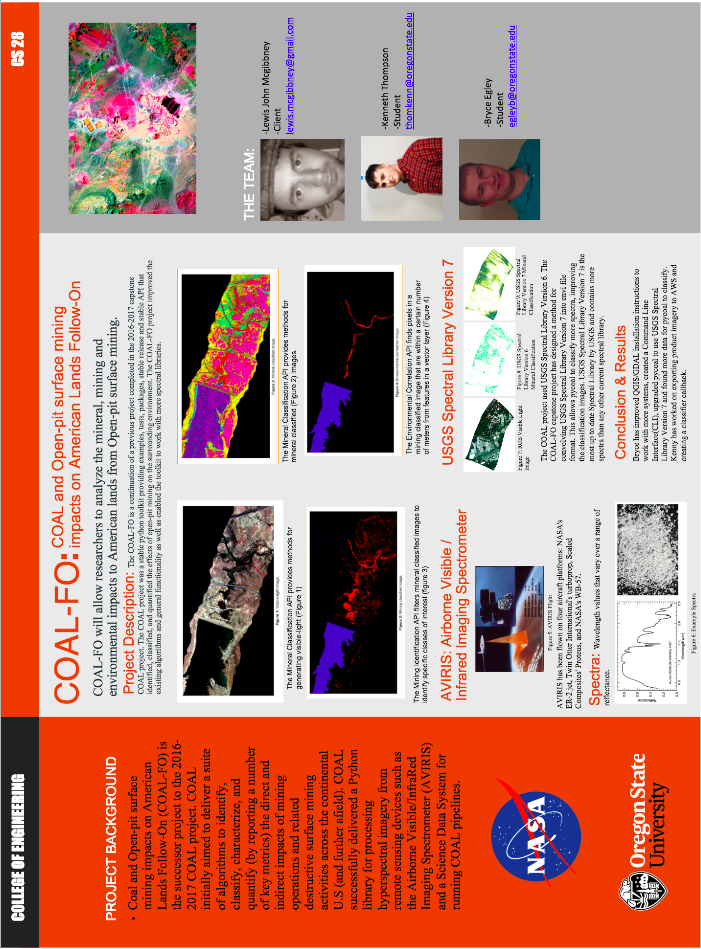
\includegraphics[width=\textwidth,height=\textheight,keepaspectratio]{Poster.png}

\section{PART 6: Project Documentation}
\subsection{How does your project work}
A very basic description of how our project works is that pycoal consumes images from AVIRIS and AVIRIS-NG. Which are infrared images picking up on a range of wavelengths over a swath of land. Pycoal also consumes a convolved Spectral Library file. Spectral Libraries contain values of light reflectance vs wavelength for hundreds of thousands of minerals or spectra. Pycoal matches up the wavelengths in the images from AVIRIS and AVIRIS-NG to the values in the convolved Spectral Library files to determine what minerals are present in the specified AVIRIS image. We then do mining and environmental correlations where we narrow down our focus to a few specific spectra or minerals and compare those to streams and other environmental features in the surrounding area.

\subsection{Theory of Computation}
Our project could be used for lots of different uses. The intent theory of operation is for looking at the impact Coal and Open pit surface mining has on surrounding lands. As well as monitoring impact of of Coal and Open pit surface mining over time. 

\subsection{How does one install your software, if any?}
First git clone pycoal from github repo \href{https://github.com/capstone-coal/pycoal}{Pycoal} and follow installation instructions and get the dependencies on \href{https://capstone-coal.github.io/docs}{ReadTheDocs}. It might be useful to also follow the instructions in the example readme \href{https://github.com/capstone-coal/pycoal/tree/master/examples}{Capstone github}. 

Pycoal works by taking infrared images from AVIRIS or AVIRIS-NG. Data Portal \href{https://avirisng.jpl.nasa.gov/alt_locator/}{here} . Downloadable Data \href{ftp://avng.jpl.nasa.gov/}{here}. Once you find data you want to download on the data portable go to the year in \href{ftp://avng.jpl.nasa.gov/}{Data Portal}. and find the file your looking for by it’s name.

\subsection{How does one run it?}
The AVIRIS file needs to be downloaded to the pycoal directory.  After building pycoal and following installation instructions, then run the classification files in the examples directory or the CLI if you choose the non default AVIRIS image.  Note** AVIRIS files are huge most ranging from 1-50GB. Running a mineral correlation on pycoal will take hours to days. In general I’ve seen that every 8 GB in size will be a full day(24 hours), but this may very on your computer.

\subsection{Are there any special hardware, OS, or runtime requirements to run your software?}
The AVIRIS files are very large. 1-50GB you will want to have a computer with at least 30GB of available storage to use pycoal. 

\subsection{Any user guides, API documentation, etc.}
\href{http://pycoal.readthedocs.io/en/latest/}{ReadTheDocs} 

\section{PART 7: Recommended Technical Resources for Learning More}
\subsection{What web sites were helpful? (Listed in order of helpfulness)}
\url{https://github.com/capstone-coal/pycoal} \\
\url{https://github.com/capstone-coal/pycoal} \\
\url{https://github.com/capstone-coal} \\
\url{https://capstone-coal.github.io/} \\
\url{https://speclab.cr.usgs.gov/spectral-lib.html} \\
\url{https://speclib.jpl.nasa.gov/} \\
\url{https://ecosis.org/} \\
\url{http://www.gdal.org/} \\
\url{https://qgis.org/en/site/} \\
\url{https://www.python.org/} \\
\url{https://aws.amazon.com/} \\

\subsection{Were there any people that were really helpful?}
\href{https://github.com/lewismc}{Lewis John McGibbney} (For question on pycoal, coal-sds or capstone website)
\href{https://www.usgs.gov/staff-profiles/raymond-kokaly?qt-staff_profile_science_products=0#qt-staff_profile_science_products}{Raymond Kokaly} (For questions on USGS Spectral Libraries)

\section{PART 8: Conclusions and Reflections (each team member answers all questions individually)}
\subsection{What technical information did you learn?}
I learned a lot more about the python language, how to convolve spectral libraries, how to create a CLI, improved my skills with git, how to use GDAL and QGIS to view hyper spectral imagery. 
\subsection{What non-technical information did you learn?}
Better time management, quickly reading through large amounts of code and figuring out what it does. Improved my skills with working in a team. 
\subsection{What have you learned about project work?}
I have learned that project work tends to take a lot longer than individual work since you don’t just need to meet your concerns and expectations but everyones in the group. As well as get approval from everyone in the group. 
\subsection{What have you learned about project management?}
I have learned that project management is essential for keeping up with deadlines and not allowing yourself to get overwhelmed.
\subsection{What have you learned about working in teams?}
I have learned that working in teams can make working on large project easier by dividing up the work amongst team members. 
\subsection{If you could do it all over, what would you do differently?}
We spent a lot of time at the start on documentation. I think the day we got assigned the project we should have tried to use all the existing code. It took about a month for me to figure how to use the entire pycoal package and install it on my computer and do a complete mineral, mining and environmental classification. At the very start we were focused too much on documentation. We also really needed three people maybe even four for a project of this size. 
\\
We also over committed at the start of the project. I think familiarizing ourselves with all of the different parts of the existing code earlier than we did would have helped with this. 

\section{PART 9: Appendix 1: Essential Code Listings}

USGS Spectral Library Version 7 conversion code \newline
\begin{lstlisting}
class FullSpectralLibrary7Convert:
    def __init__(self):
        """
            This class method converts the entire `USGS Spectral Library Version 7
            <https://speclab.cr.usgs.gov/spectral-lib.html>`_ library into
            its convolved envi format

            Args:
            none
            """
        pass

    @classmethod
    def convert(cls, library_filename=""):
        """
            This class method converts the entire `USGS Spectral Library Version 7
            <https://speclab.cr.usgs.gov/spectral-lib.html>`_ library into
            its convolved envi format

            Spectral Library Version 7 can be downloaded `here <https://speclab.cr.usgs.gov/spectral-lib.html>`_

            Args:
            library_filename (str): path to USGS Spectral Library Version 7 directory
            """
        if not library_filename:
            raise ValueError("Must provide path for USGS Spectral Library Version 7.")

        #This will take all the necessary .txt files for spectra in USGS
        #Spectral Library Version 7 and put them in a new directory called
        #"usgs_splib07_modified" in the examples directory
        directory = 'usgs_splib07_modified'
        if not os.path.exists(directory):
            os.makedirs(directory)

        for root, dir, files in os.walk(library_filename + "/ASCIIdata"):
            dir[:] = [d for d in dir]
            for items in fnmatch.filter(files, "*.txt"):
                if "Bandpass" not in items:
                    if "errorbars" not in items:
                        if "Wave" not in items:
                            if "SpectraValues" not in items:
                                shutil.copy2(os.path.join(root,items), directory)

        #This will take the .txt files for Spectra in USGS Spectral Version 7 and
        #convert their format to match that of ASTER .spectrum.txt files for spectra
        # create a new mineral aster conversion instance
        spectral_aster = SpectalToAsterFileFormat()
        #List to check for duplicates
        spectra_list = []
        # Convert all files
        files = os.listdir(directory +'/')
        for x in range(0, len(files)):
            name = directory+'/' + files[x]
            #Get name
            input_file = open(name,'r')
            spectra_line = input_file.readline()
            spectra_cut = spectra_line[23:]
            spectra_name = spectra_cut[:-14]
            #Remove first and last char in case extra spaces are added
            spectra_first_space = spectra_name[1:]
            spectra_last_space = spectra_first_space[:-1]

            #Check if Spectra is unique
            set_spectra = set(spectra_list)
            if not any(spectra_name in s for s in set_spectra):
                if not any(spectra_last_space in a for a in set_spectra):
                    spectral_aster.convert(name)
                    spectra_list.append(spectra_name)

        set_spectra = set(spectra_list)
        print(set_spectra)

        #This will generate three files s07av95a_envi.hdr, s07av95a_envi.hdr.sli,splib.db and dataSplib07.db
        #For a library in `ASTER Spectral Library Version 2.0 <https://asterweb.jpl.nasa.gov/>`_ format
        data_dir = "dataSplib07.db"
        header_name = "s07_AV95_envi"

        # create a new mineral aster conversion instance
        spectral_envi = AsterConversion()
        # Generate .sli and .hdr
        spectral_envi.convert(directory,data_dir,header_name)
\end{lstlisting}
Code for unit tests of USGS Spectral Library 7 conversion function
\newline
\begin{lstlisting}
# test files for FullSpectralLibrary7Convert conversion test
_test_SpectralConversion_data = 'usgs_splib07'
_test_SpectralConversion_dir = 'usgs_splib07_modified'
_test_SpectralConversion_db = 'dataSplib07.db'
_test_SpectralConversion_envi = 's07_AV95_envi'

# tear down FullSpectralLibrary7Convert conversion test by deleting test files
def _test_spectral_conversion_teardown():
    _remove_files([_test_SpectralConversion_db,
                   _test_SpectralConversion_dir])

# verify that a small subset of the USGS Spectral Library 7 is converted to ENVI format
@with_setup(None, _test_spectral_conversion_teardown)
def test_spectral_conversion():
    data, dir, db, envi = _test_SpectralConversion_data, _test_SpectralConversion_dir, _test_SpectralConversion_db, _test_SpectralConversion_envi
    spectral_conversion = mineral.FullSpectralLibrary7Convert()
    spectral_conversion.convert(library_filename=data)
    spectral7 = spectral.open_image(envi+'.hdr')
    assert isinstance(spectral7, spectral.io.envi.SpectralLibrary)
\end{lstlisting}

\section{PART 10: Appendix 2: Anything else you want to include. Photos, etc.}

I had to remove photos since the engineering server did not accept images in Latex.
\newline
I included the images in in the images folder
\newline
USGS Spectral Library version 6 classification image is images 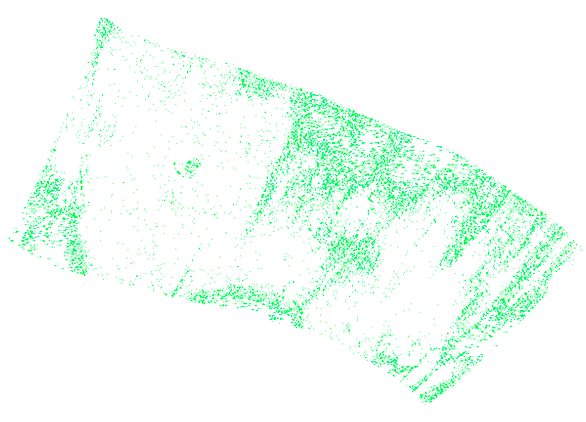
\includegraphics[width=.6\textwidth,left]{images/S061.png}
\newline
USGS Spectral Library version 7 classification image is images 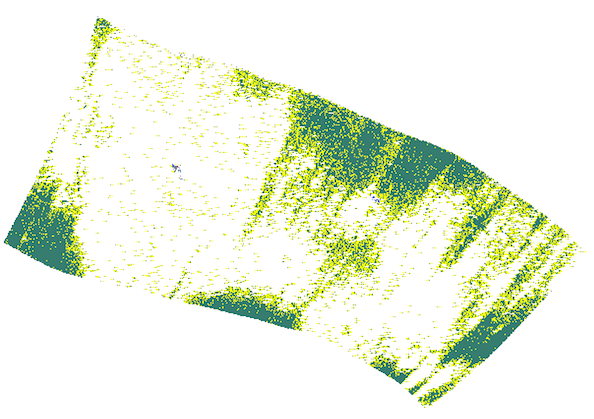
\includegraphics[width=.6\textwidth,left]{images/S071.png}
\newline
USGS Spectral Library version 6 classification of San Juan Coal Mine is 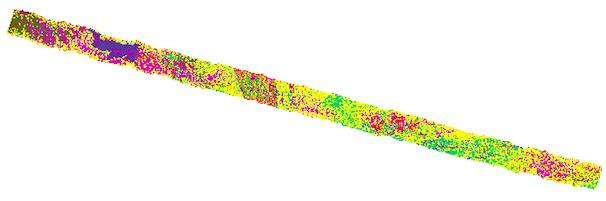
\includegraphics[width=.6\textwidth,left]{images/S062.png}
\newline
USGS Spectral Library version 7 classification of San Juan Coal Mine is 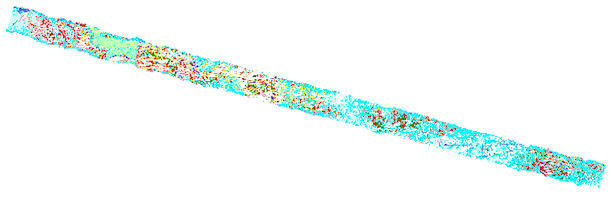
\includegraphics[width=.6\textwidth,left]{images/S072.png}

\begin{thebibliography}{9}
\bibitem{1} ”CS461 - CS Senior Capstone”, Eecs.oregonstate.edu, 2017. [Online]. Available: \url{http://eecs.oregonstate.edu/capstone/cs/capstone.cgi?project=320} [Accessed: 22- Nov- 2017]

\bibitem{2} ”USGS.gov — Science for a changing world”, Usgs.gov, 2017. [Online]. Available: \url{https://www.usgs.gov/} [Accessed: 22- Nov- 2017]

\bibitem{3} ]”AVIRIS - Airborne Visible / Infrared Imaging Spectrometer”, Aviris.jpl.nasa.gov, 2017. [Online]. Available:
\url{https://aviris.jpl.nasa.gov/} [Accessed: 22- Nov- 2017].

\bibitem{4} ”XSEDE User Portal — Globus User Guide”, Portal.xsede.org, 2017. [Online]. Available: \url{https://portal.xsede.org/software/globus} [Accessed: 22- Nov- 2017].

\bibitem{5} ”C++”, En.wikipedia.org, 2017. [Online]. Available:
\url{https://en.wikipedia.org/wiki/C} [Accessed: 22- Nov- 2017].

\bibitem{6} "MySQL", En.wikipedia.org, 2017. [Online]. Available: \url{https://en.wikipedia.org/wiki/MySQL} [Accessed: 22- Nov- 2017].

\bibitem{7} "XSEDE, Extreme Science and Engineering Discovery Environment", www.xsede.org, 2017. [Online]. Available: \url{https://www.xsede.org/} [Accessed: 22- Nov- 2017].

\bibitem{8} "AVIRIS, Airborne Visible/Infrared Imaging Spectrometer", aviris.jpl.nasa.gov, 2017. [Online]. Available: \url{https://aviris.jpl.nasa.gov/} [Accessed: 22- Nov- 2017].

\bibitem{9} "AVIRIS-NG, airborne Visible/Infrared Imaging Spectrometer Next Generation", aviris-ng.jpl.nasa.gov, 2017. [Online]. Available: \url{https://aviris-ng.jpl.nasa.gov/}[Accessed: 22- Nov- 2017].

\bibitem{10} "COAL, Coal and Open-pit surface mining impacts on American Lands", capstone-coal.github.io, 2017. [Online]. Available: \url{https://capstone-coal.github.io/} [Accessed: 22- Nov- 2017].

\bibitem{11} "HPC, High Performance Computing", en.wikipedia.org, 2017. [Online]. Available: \url{https://en.wikipedia.org/wiki/Supercomputer} [Accessed: 22- Nov- 2017].

\bibitem{12} "Query Language", en.wikipedia.org, 2017. [Online]. Available: \url{https://en.wikipedia.org/wiki/Query_language} [Accessed: 22- Nov- 2017].

\bibitem{13} "Enterprise Module Service", hpccsystems.com, 2017. [Online]. Available: \url{https://hpccsystems.com/enterprise-services/modules/esp} [Accessed: 22- Nov- 2017].

\bibitem{14} "HPCC High Performance Computing Cluster", hpccsystems.com, 2017. [Online]. Available: \url{https://hpccsystems.com/enterprise-services/modules/esp} [Accessed: 22- Nov- 2017].

\bibitem{15} "OSU Unix HPC Cluster", cosine.oregonstate.edu, 2017. [Online]. Available \url{http://cosine.oregonstate.edu/unix-hpc-cluster} [Accessed: 22- Nov- 2017].

\bibitem{16} "MIT License", en.wikipedia.org, 2017. [Online]. Available: \url{https://en.wikipedia.org/wiki/MIT_License} [Accessed: 29- Nov- 2017].

\bibitem{17} "Apache License Version 2.0", www.apache.org, 2017. [Online]. Available \url{https://www.apache.org/licenses/LICENSE-2.0} [Accessed: 29- Nov- 2017].

\bibitem{18} "GNU General Public License, version 2", www.gnu.org, 2017. [Online]. Available \url{https://www.gnu.org/licenses/old-licenses/gpl-2.0.en.html} [Accessed: 29- Nov- 2017].

\bibitem{19} "Top Open Source Licenses",www.blackducksoftware.com, 2017.[Online]. Available \url{https://www.blackducksoftware.com/top-open-source-licenses} [Accessed: 29- Nov- 2017].
\end{thebibliography}

\end{document}

